In this section, we present the performance of a number of policies when run with varying cost-parameter for both the AM and PM periods.  %We then first identify key take-aways from the results, and later provide analysis on these observations. 
The data-set for the test period, on which our analysis relies, consists of a total of 4944 trips in the AM and 2800 trips in the PM, across 147 stations. We focus our analysis on the deterministic regime in which we assume that an incentivized rental/return is always triggered by the incentive given and would not have occurred otherwise. Thereafter, we contrast those results with the ones in the stochastic regime. The scores for the former are displayed in Table \ref{table:det} and for the latter in Table \ref{table:stoch}. All scores are given as the fraction of improvement of the % evaluation and later provide analysis on the stochastic evaluation results. The deterministic performance scores for both the morning (AM) and afternoon (PM) are presented in Table [1], and the scores are relative scores compared to the perfectly 
optimal dynamic policy (i.e., each policy's absolute score is divided by the dynamic policy's absolute score). We begin by giving a high-level summary of our most interesting findings before providing more details for each of them.

%In this section, we present and analyze both the deterministic and stochastic performance results of the different policies when run with various cost parameters. The overall analysis is performed on a total of 147 incentive stations during the test period, which accounts to a total of 4944 AM trips and 2800 PM trips. In the next subsections, we will first identify key take-aways from the deterministic results, and provide analysis on these observations. Afterwards, we will examine the stochastic results and what they indicate. The deterministic and stochastic performance results are presented in Table 1 and 2 respectively. All scores presented in both tables are relative scores compared to the optimal dynamic policy (i.e. each policy's absolute score divided by the dynamic policy's absolute score). 

\begin{table}
\caption{Policy Performance Scores in Deterministic Regime.}
\label{table:det}
\begin{tabular}{ |l| l| *5{c|}  }
\hline
\multirow{2}{*}{Time} & \multirow{2}{*}{Policies} & \multicolumn{5}{ c| }{Cost Parameter}\\  \cline{3-7}
& & 0.0 & 0.1 & 0.2 & 0.3 & 0.4 \\ \hline
\multirow{9}{*}{AM} & Dynamic & 1.0 & 1.0 & 1.0 & 1.0 & 1.0 \\
 & Stat. Opt. & 0.985  & 0.981& 0.976 & 0.97 & 0.961  \\
 & Static & 0.939  & 0.911 & 0.870 & 0.809 & 0.715 \\
 & Stat. HS & 0.960 & 0.947 & 0.929 & 0.905 & 0.873 \\ 
 & Clus. HS & 0.961 & 0.944 & 0.918 & 0.887 & 0.845 \\ 
 & Dyn 15 & 1.0 & 1.0 & 1.0 & 1.0 & 1.0\\ 
 & Dyn 30 & 0.995 & 0.994 & 0.993 & 0.992 & 0.990 \\ 
 & Dyn 60 & 0.989 & 0.984 & 0.980 & 0.977 & 0.969 \\ 
 & Dyn 120 & 0.967 & 0.953 & 0.944 & 0.940 & 0.924 \\
 \hline
\multirow{9}{*}{PM} & Dynamic & 1.0 & 1.0 & 1.0 & 1.0 & 1.0 \\
 & Stat. Opt. & 0.980 & 0.977 & 0.974 & 0.972 & 0.967\\
 & Static & 0.844 & 0.777 & 0.680 & 0.538 & 0.318 \\
 & Stat. HS & 0.943 & 0.934 & 0.917 & 0.891 & 0.858 \\ 
 & Clus. HS & 0.932 & 0.917 & 0.897 & 0.866 & 0.830 \\ 
 & Dyn 15 & 1.0 & 1.0 & 1.0 & 1.0 & 1.0 \\ 
 & Dyn 30 & 0.986 & 0.984 & 0.982 & 0.983 & 0.980 \\ 
 & Dyn 60 & 0.975 & 0.965 & 0.956 & 0.958 & 0.951 \\ 
 & Dyn 120 & 0.949 & 0.926 & 0.909 & 0.919 & 0.904 \\
 \hline
\end{tabular}
\caption*{Relative performances of each policy during AM and PM periods compared to the completely online policy under the deterministic performance evaluation.
}
\end{table}

\begin{table}
\caption{Policy Performance Scores in Probabilistic Regime.}
\label{table:stoch}
\begin{tabular}{ |l| l| *4{c|}  }
\hline
\multirow{2}{*}{Period} & \multirow{2}{*}{Policies} & \multicolumn{4}{ c| }{Cost Parameter}\\  \cline{3-6}
& & 0.0 & 0.01 & 0.1 & 0.2 \\ \hline
\multirow{9}{*}{AM} & Dynamic & 1.0 & 1.0 & 1.0 & 1.0  \\
 & Stat. Opt. & 0.979 & 0.973 & 0.945 & 0.912  \\
 & Static & 0.928 & 0.916 & 0.771 & 0.479 \\
 & Static HS & 0.957 & 0.944 & 0.878 & 0.796 \\ 
 & Clus. HS & 0.958 & 0.931 & 0.831 & 0.699 \\ 
 & Dyn 15 & 1.0 & 1.0 & 1.0 & 1.0\\ 
 & Dyn 30 & 0.995 & 0.995 & 0.993 & 0.991 \\ 
 & Dyn 60 & 0.985 & 0.870 & 0.832 & 0.773 \\ 
 & Dyn 120 & 0.966 & 0.68 & 0.612 & 0.514 \\
 \hline
\multirow{9}{*}{PM} & Dynamic & 1.0 & 1.0 & 1.0 & 1.0  \\
 & Stat. Opt. & 0.978 & 0.971 & 0.943 & 0.917  \\
 & Static & 0.923 & 0.903 & 0.646 & 0.15 \\
 & Stat. HS & 0.967 & 0.948 & 0.883 & 0.784 \\ 
 & Clus. HS & 0.958 & 0.935 & 0.839 & 0.682 \\ 
 & Dyn 15 & 1.0 & 1.0 & 1.0 & 1.0\\ 
 & Dyn 30 & 0.992 & 0.990 & 0.992 & 0.99 \\ 
 & Dyn 60 & 0.982 & 0.889 & 0.850 & 0.807 \\ 
 & Dyn 120 & 0.960 & 0.823 & 0.756 & 0.702 \\
 \hline
\end{tabular}
\caption*{Relative performance of each policy during AM and PM periods compared to the completely online policy under the probabilistic performance evaluation.}
\end{table}



\subsection{Key Observations of Deterministic Results}
Considering the rows indexed by Static for both AM and PM periods and both tables, it is noticeable that the static policy performs quite well, especially in the regime with low cost parameters, which is strong evidence of the operator's domain expertise in the initial choice of incentivized stations. Next, we observe the near-optimal performance of the Static Optimal benchmark across all cost parameters; this supports our decision to restrict the offline policies to  incentivize only over sub-intervals. For the dynamic policies, we observe a smooth decrease in performance as we transition from the maximally dynamic to more static policies, which highlights the trade-offs between efficiency and simplicity in the policies. Noticeably, none of the offline policies handle high cost-parameters well. Last, we observe a general decrease in performance from the AM to PM period, indicating that the system behavior is more erratic in the afternoon.
 
\subsubsection{Static Performance}
At first glance, the strong performance of the Static policy in Table \ref{table:det} (0.939 in the AM without costs) may seem surprising. It is explained, however, by the operator's domain expertise when deciding which stations to include in the incentive scheme. Its degrading performance with increased costs is explained by the fact that the policy does not adapt to the shrinking set of trips with positive impact as costs increase.
%In considering the Static policy's results in Table 1, it is interesting to note the policy's strong performance with no cost parameters, scoring up to 0.939 in the AM period. In hindsight, this is not surprising and exemplifies Citi Bike's domain expertise when setting the initial incentive policy. Likewise, the degrading performance with increased costs is unsurprising, since the policy does not adapt to the shrinking set of trips with positive impact as the cost increases. % shrink with higher costs.

Despite its reasonable performance in the AM in the regime without costs, the Static policy is still dominated by all policies across  all cost parameters. This is especially prominent in the PM period, where differences range from 9\% (Stat. HS)  up to 15\% (Dyn 15) even without cost parameters; the differences are even higher when accounting for costs. All of the incentivized trips in the PM, grouped by their improvement on the objective, $\delta_r$, are visualized in Figure \ref{fig:Static Performance}. Though the vast majority of incentivized trips have positive-impact, the other policies are able to accurately exclude those trips that do not, thus achieving higher performance.  These results exemplify the importance of a data-driven approach to improve the Bike Angels program. For example, even a rather simple policy with minimal overhead, such as Static Hindsight, significantly improves the efficiency of the incentives.

\begin{figure}
\centering
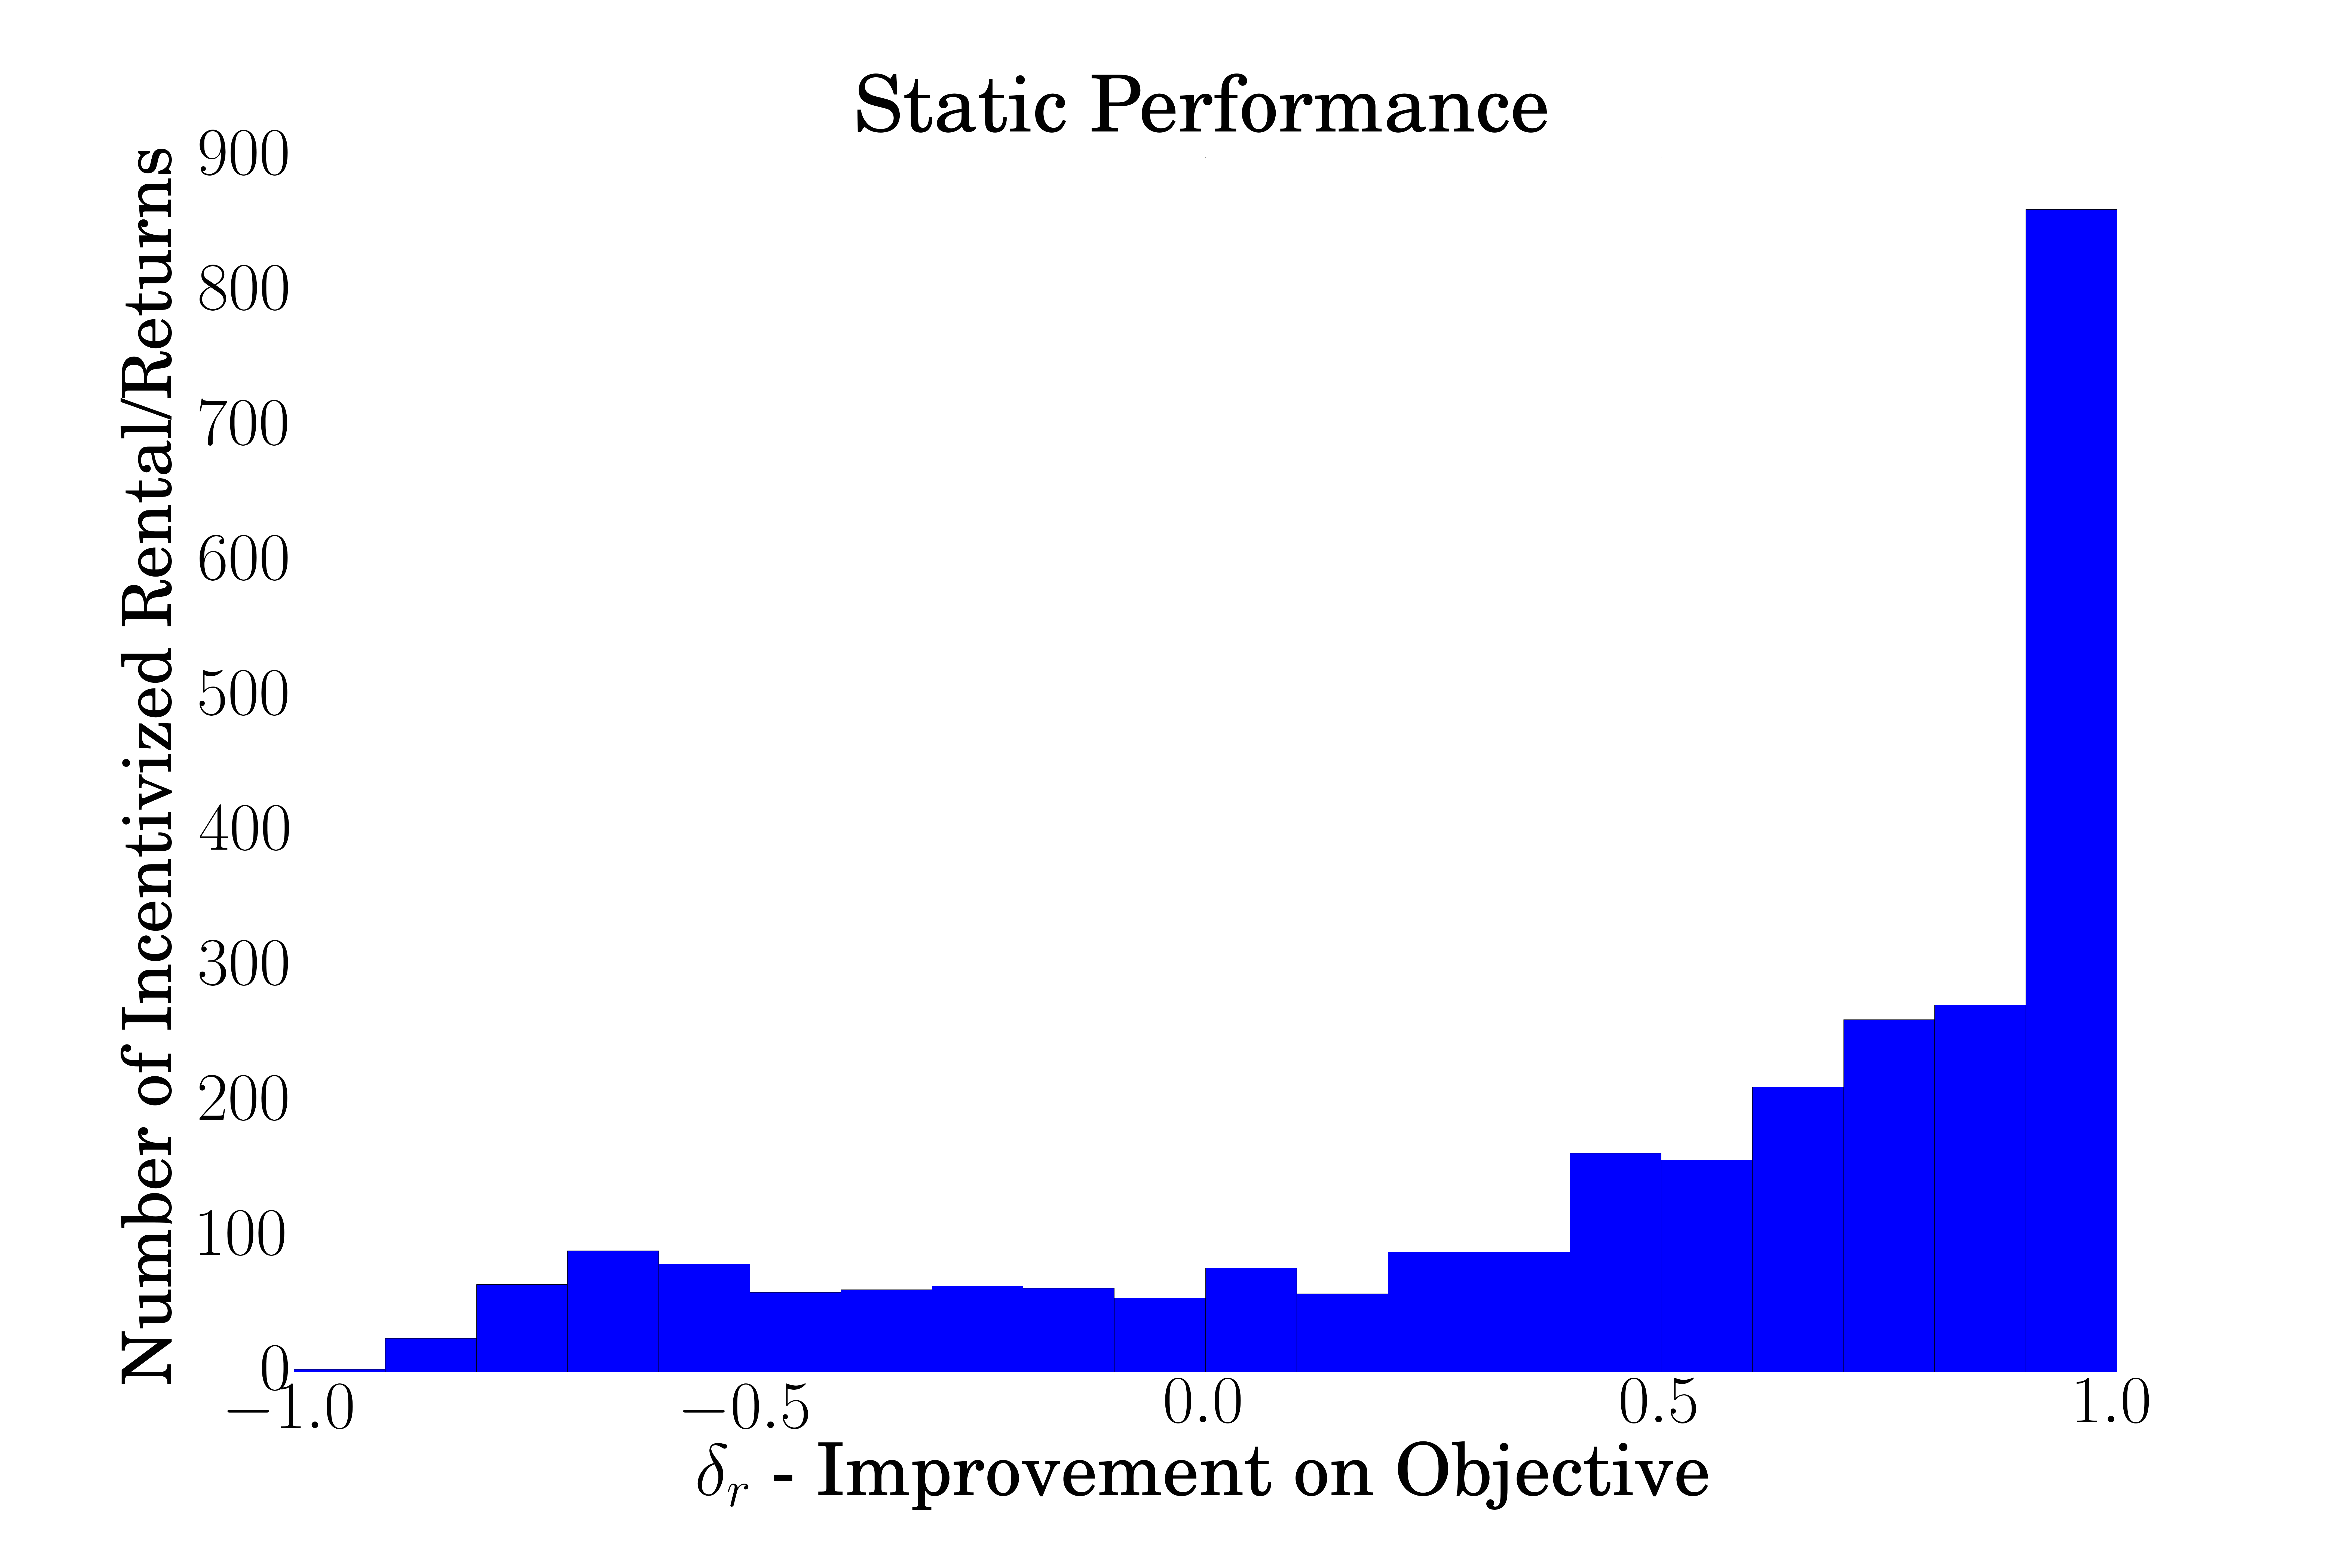
\includegraphics[width=.5\textwidth]{../SubmissionPlots/ActuallyUsed/Static_Performance_PM.png}
\caption{Static Policy's total number of incentivized trips, grouped by impact on objective ($\delta_r$) for the PM period.}
\label{fig:Static Performance}
\end{figure}


%Original text.
%This exemplifies the importance of a data-driven approach to improve the Bike Angels program. For example, even a rather simple policy with minimal overhead, such as Static Hindsight, significantly improves the efficiency of the incentives.

\subsubsection{Static Optimal Benchmark Performance}
The online policies have two advantages over the offline policies: the flexibility to adapt decisions with updated information and the flexibility to incentivize over periods that are not sub-intervals. Comparing the performance of the Static Optimal to the Dynamic policy helps us  distinguish between these two effects. More specifically, the benchmark operates with perfect information but is constrained to only incentivize over sub-intervals. %Thus if the benchmark performs near-optimal, it suggests subinterval incentives are reasonable, and vice versa.

In Table \ref{table:det} we do indeed observe Static Opt achieving a near optimal score of 0.98, which only slightly worsens with increased costs. This supports our assumption that it suffices to incentivize over a single sub-interval. However, Static Opt assumes perfect knowledge and still only matches the performance of Dynamic CC (60). In that sense, it also demonstrates the limitations of the best feasible offline policies.

\subsubsection{Online to Offline Policies}
Unsurprisingly, we find that the online policies outperform offline policies. As we transition from the maximally dynamic and online policy to the entirely static and offline policy, the decrease in performance occurs in a somewhat smooth way. % show an interesting smooth decrease in performance as we . If we imagine placing the policies on a dynamic/static spectrum, with Dynamic on one end and Static on the other, the results exemplify the continuous trade-offs between efficiency and simplicity as we move along the spectrum. Concrete examples of this trade-off in terms of the operator and user's experience is the following: with more dynamic online policies the incentives are more efficient; however, this comes at the cost of simplicity for the operator in terms of the increased IT set-up, and for the user in terms of the undesirable reduced predictability on where incentives will be given in the future. 

An interesting result in this context is the performance of the Dynamic CC (15) policy in Tables \ref{table:det} and \ref{table:stoch}, as it achieves optimal scores for all sets of parameters; this demonstrates that making decisions completely online/in real time is not necessary to obtain perfect efficiency.

On the other end of the spectrum from online to offline, the results of Table \ref{table:det} demonstrate that the offline policies Static Hindsight and Cluster Hindsight perform almost on par with the online Dynamic CC (120) policy, especially in the regime with low cost parameters; this points to the limited advantage of the simple online policies as the cost parameter increases. %This indicates that the benefits of an online policy with dynamic decision making is almost insignificant at this point of the dynamic/static spectrum.

\subsubsection{The Cost Parameter}
%New
In considering the relative performance change of policies with increasing cost parameters, we find that the offline policies are comparatively much worse at handling high cost parameters than the online policies. Intuitively, it might seem that the interval incentive restrictions of offline policies leads to this result. For example, imagine taking the original incentive interval with no cost parameter, and changing some of the positive-impact trips within the interval to become negative-impact trips (due to increase in cost). Then unless these trips all exist at the outer limits of the interval, these trips will "shatter" the incentive interval: either the offline policies give up on the positive-impact trips at the beginning or they give up on the positive-impact trips at the end or they include the negative-impact trips in the middle. Online policies on the other end can avoid this conundrum as they are not restricted to a single sub-interval. 

However, the performance of the Static Optimal benchmark in Table \ref{table:det} does not significantly degrade with high cost parameters. Thus, despite the interval restriction, the offline policies still have room to have better predictions yield improved performance.

In contrast, Figure \ref{fig: Dynamic CC 60 Policy} displays for the Dynamic CC (60) all incentivized trips with their time of day, their expected impact on future out-of-stock events, and for each one, the decision whether or not it is incentivized when run with 2 different cost parameters.% within nicely illustrates how the dynamic policies adapt to increased cost parameters. % shows the c of Dynamic CC 60 as cost parameters are increased from 0.0 to 0.3. The top scatter plot indicates for each incentivized trip, indexed by time of trip and $\delta_r$, whether it is included/excluded in the Dynamic CC 60 policy incentivization under a 0.0 cost parameter regime. The bottom plot is the same plot except when the cost parameter is increased to 0.3. 
The cost parameter is specified in each plot by the y-value of the horizontal line dividing the positive-impact trips (above the line) and negative-impact trips (below the line). As the cost parameter increases from 0.0 to 0.3, the policy excludes most trips having a $\delta_r$ value between that range, that it had previously included. Thereby, it manages to retain its near-optimal performance.



%The efficiency of online policies even with increasing cost parameters can be seen in the two scatter plots of Figure 4, that indicate which incentivized trips are included/excluded in the Dynamic CC 60 policy under low (0.0) and high (0.3) cost parameter regimes. The trips are indexed by time of day on the x-axis and $\delta_r$ value on the y-axis, and the cost parameter is specified by the y-value of the horizontal line dividing the positive-impact (above the line) and negative-impact (below the line) trips for the respective cost. The figure shows how the Dynamic CC 60 policy gracefully handles the increase in cost parameter from 0.0 to 0.3 by excluding most trips it had previously included with a $\delta_r$ value between that range.


\begin{figure}
\centering

 \begin{subfigure}{\textwidth}
 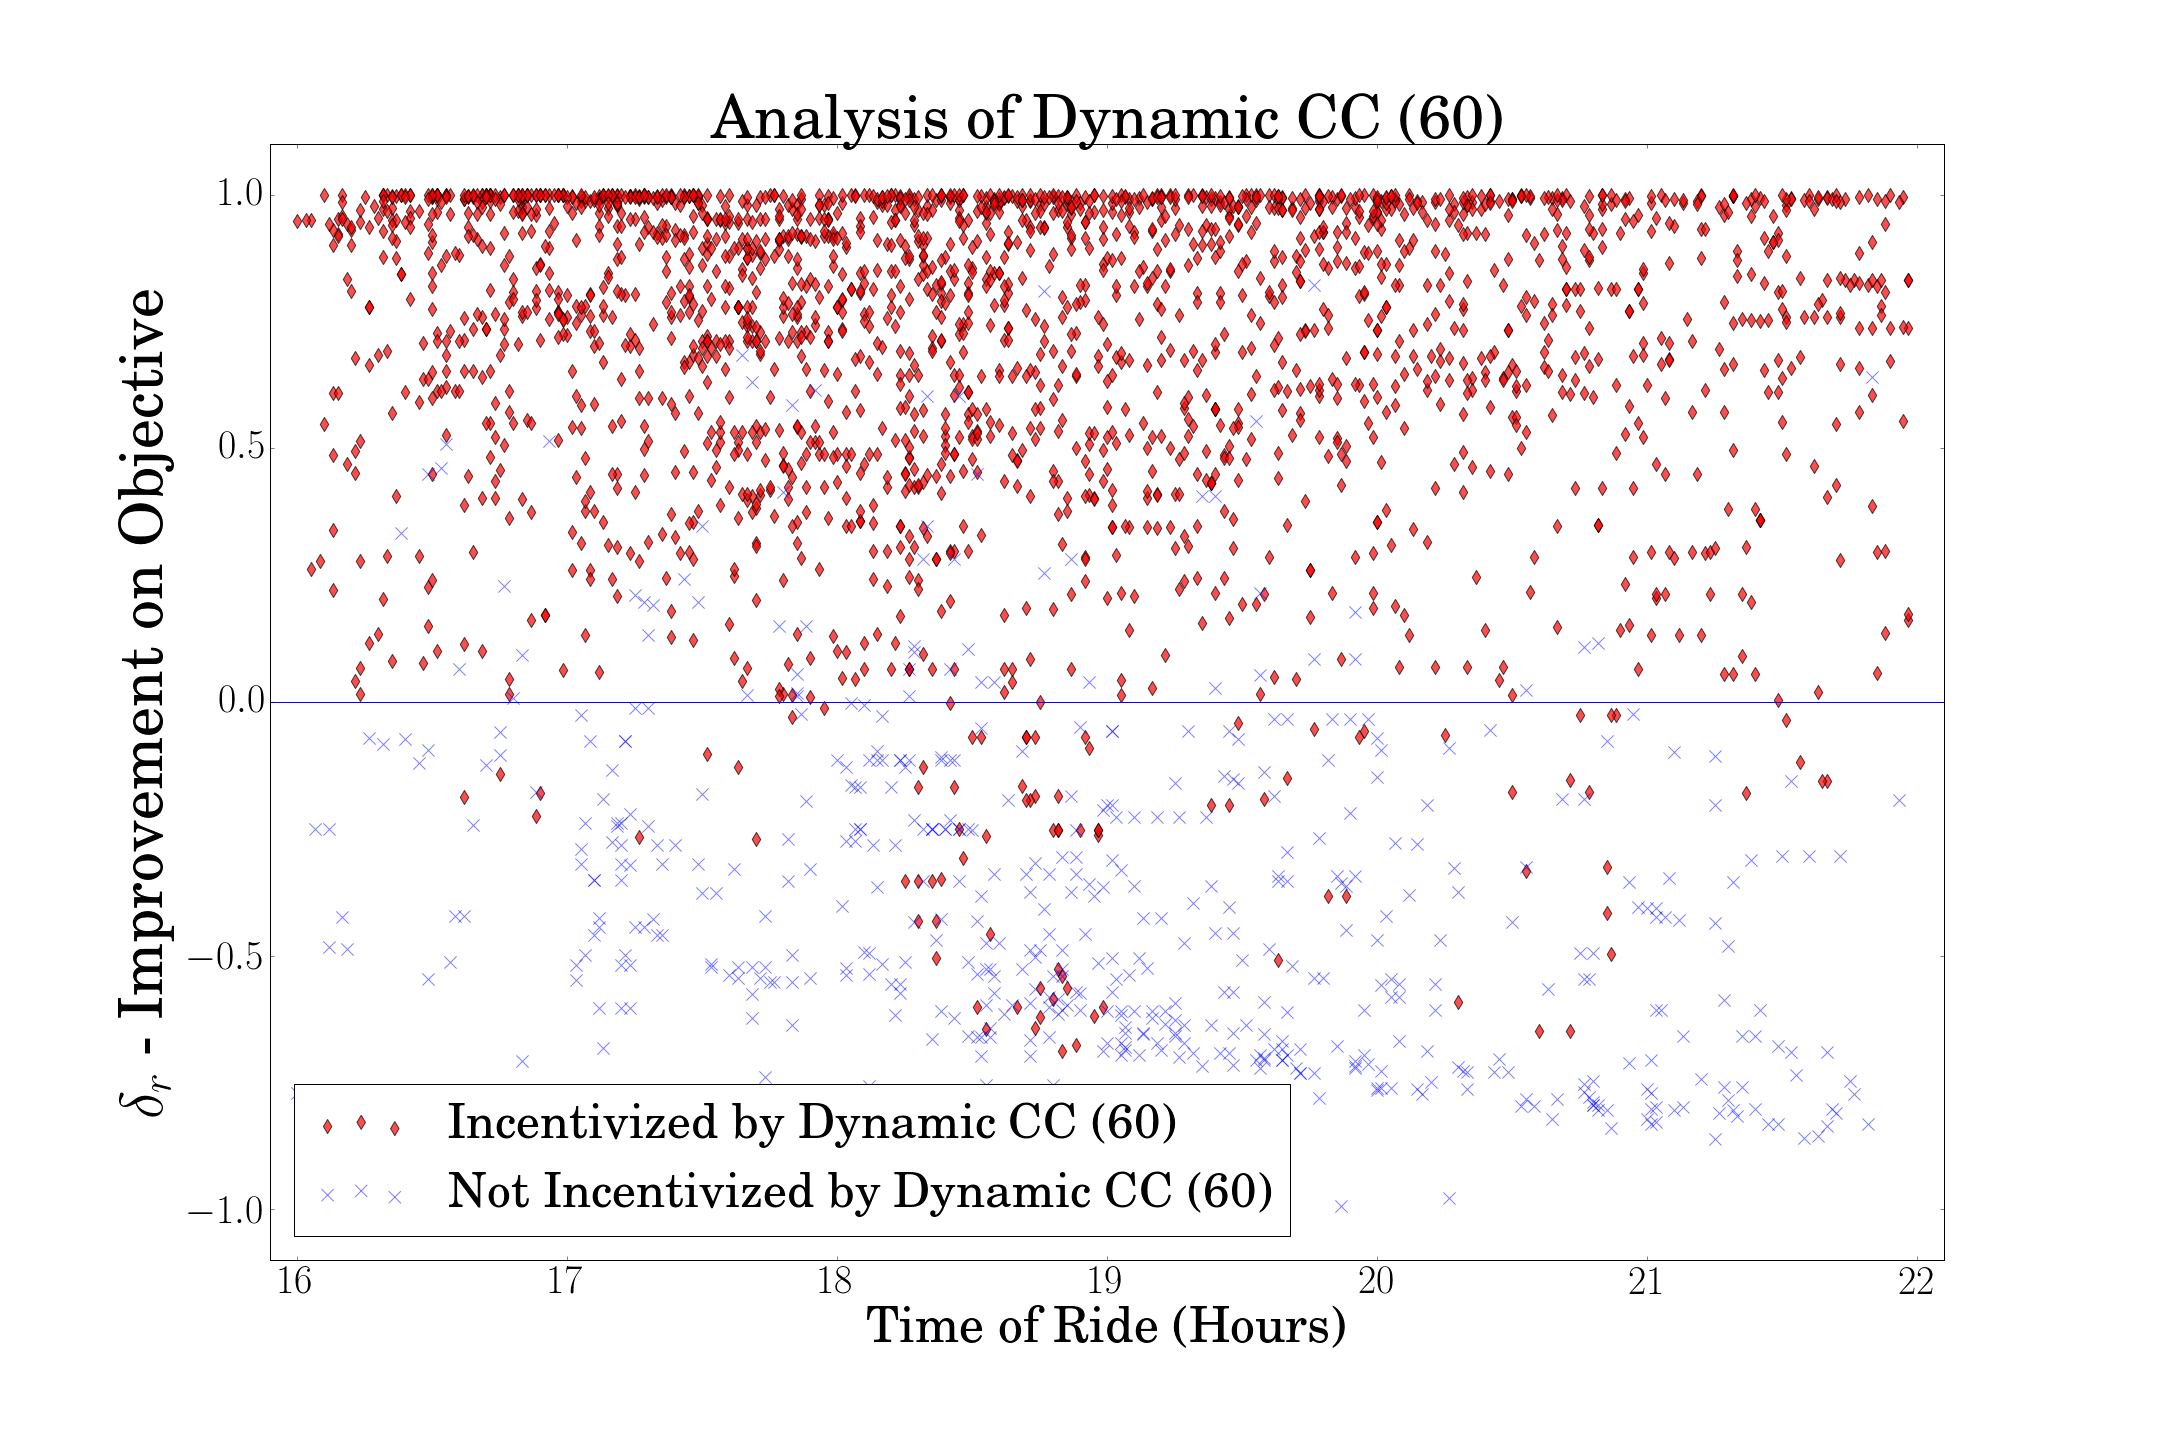
\includegraphics[width=.5\textwidth]{../SubmissionPlots/ActuallyUsed/scatter_60_0.png}
 \end{subfigure}
 \begin{subfigure}{\textwidth}
 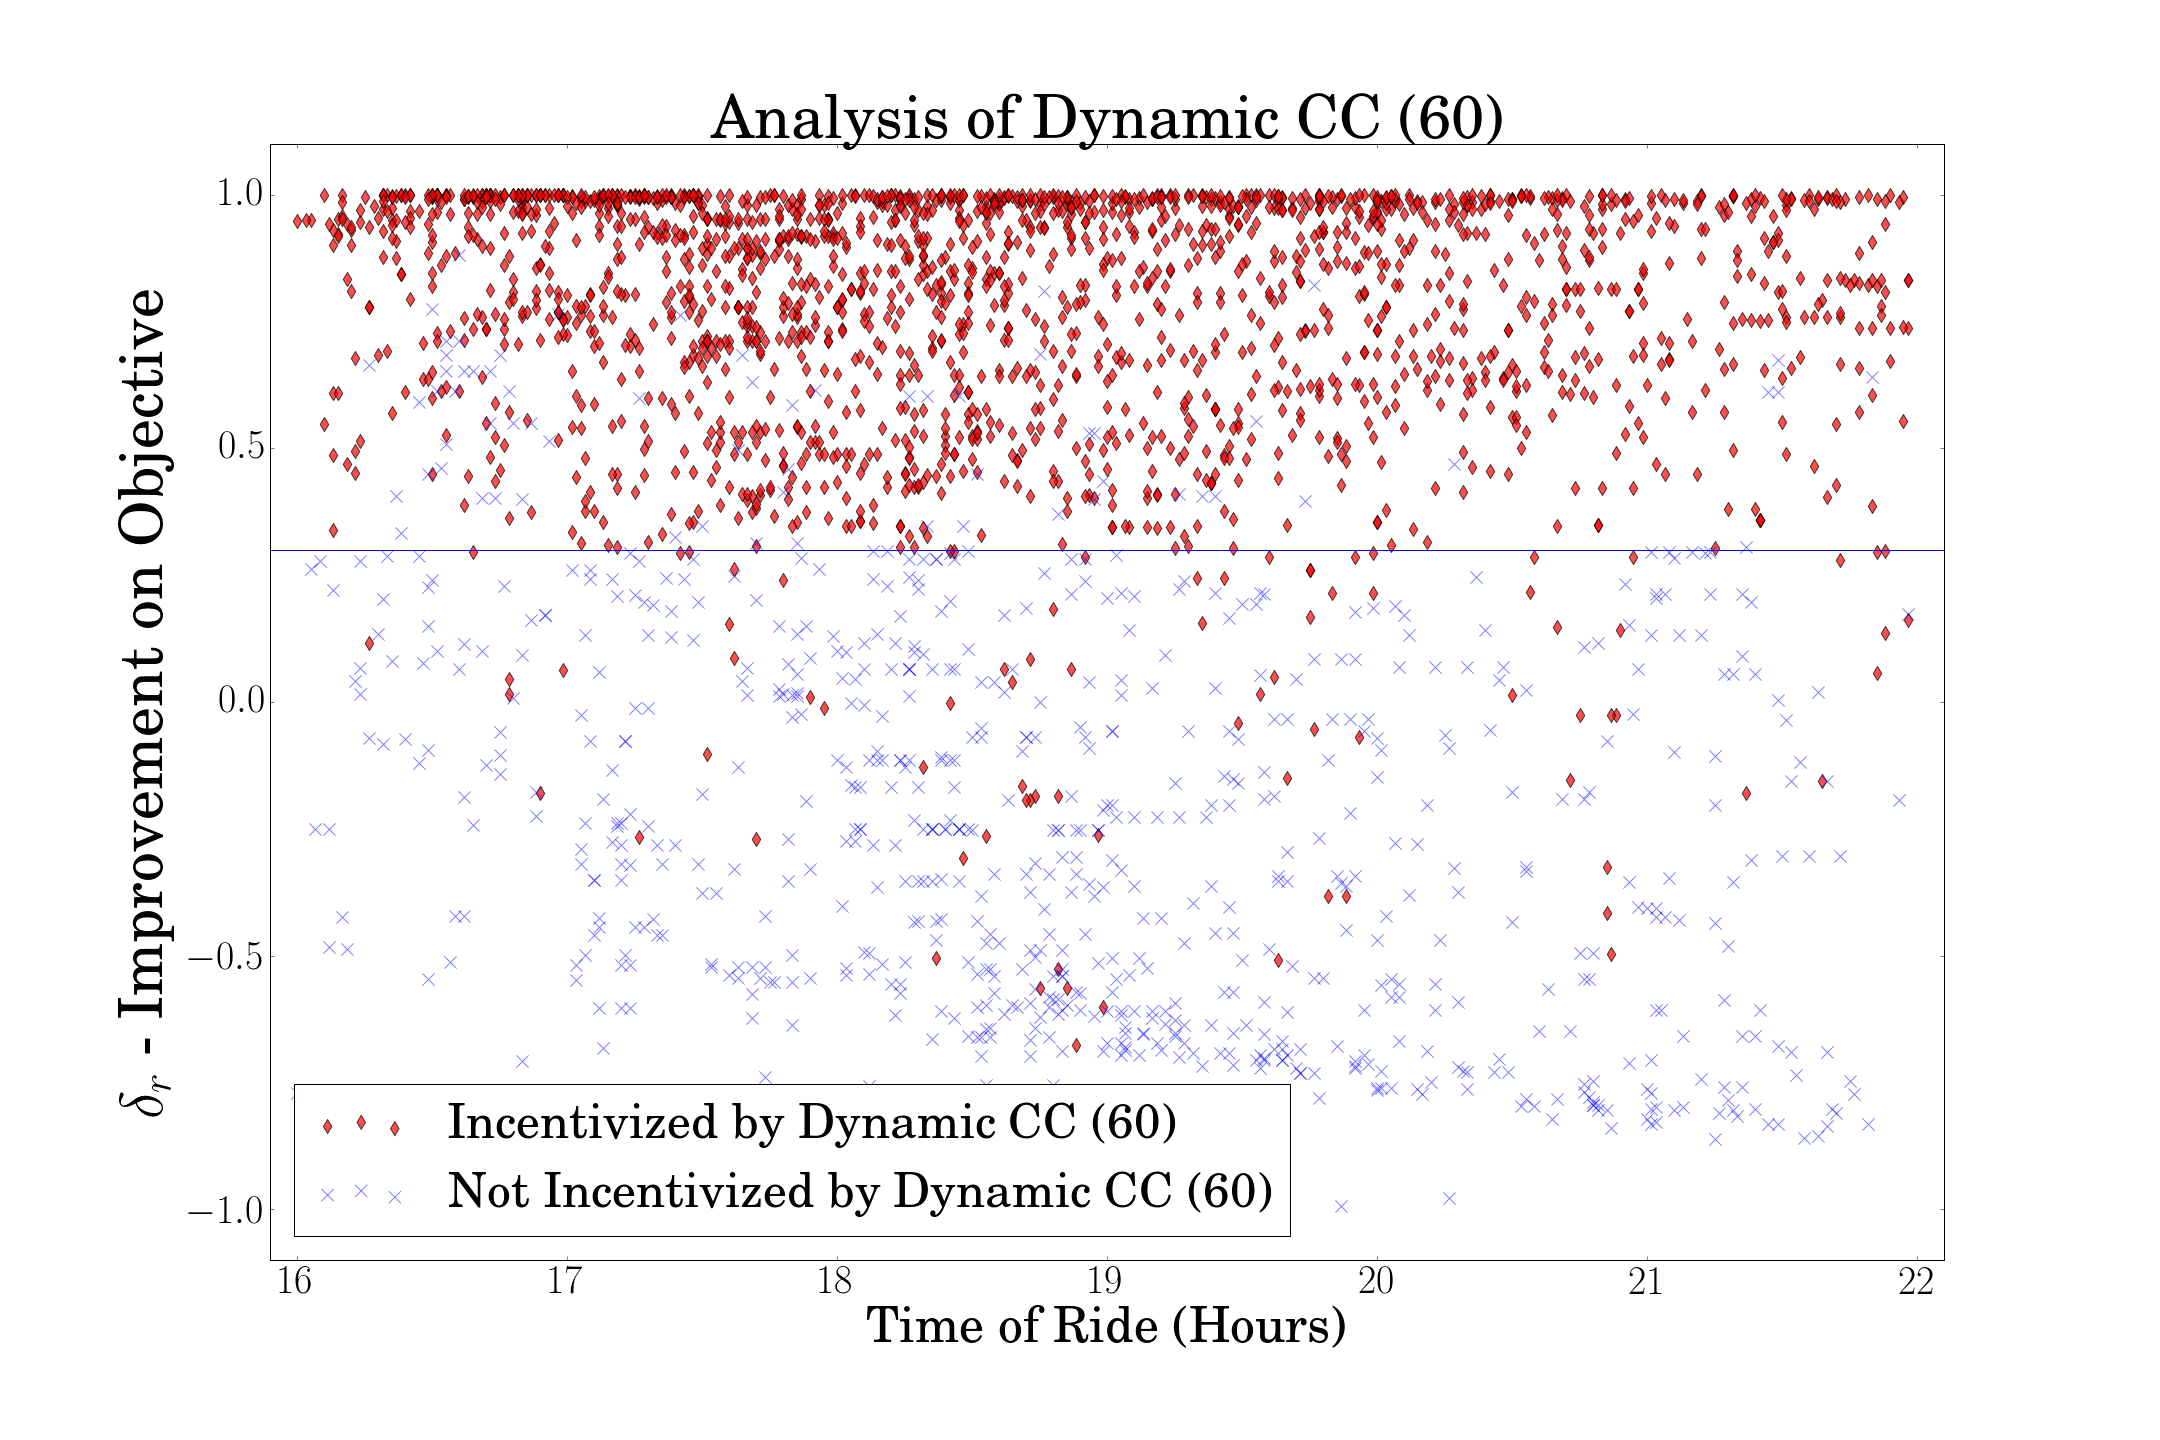
\includegraphics[width=.5\textwidth]{../SubmissionPlots/ActuallyUsed/scatter_60_3.png}
 \end{subfigure}
 
 \caption{Scatter plots of incentivized trips indicating which trips are included/excluded in Dynamic CC (60) incentivization policy, when cost parameter is 0.0 (top) and 0.3 (bottom).}

\label{fig: Dynamic CC 60 Policy}
\end{figure}


%Before
%In considering the relative performance change of policies with increasing cost parameters, we find that the offline policies are comparatively much worse at handling high cost parameters than the online policies. Intuitively, it might seem that the inherent interval incentive restrictions of offline policies leads to this result. For example, imagine taking the original incentive interval with no cost parameter, and changing some of the positive-impact trips within the interval to become negative-impact trips (due to increase in cost). Then unless these trips all exist at the outer limits of the interval, these trips will "shatter" the incentive interval: either the offline policies give up on the positive-impact trips at the beginning or they give up on the positive-impact trips at the end or they include the negative-impact trips in the middle. Online policies on the other end can avoid this conundrum as they are not restricted to a single sub-interval. However, the performance of the Static Optimal benchmark in Table \ref{table:det} does not significantly degrade with high cost parameters, indicating that even with the interval restriction, the offline policies still have room to have better predictions yield improved performance. %inability of offline policies to handle high cost parameters is due not only to the interval restriction, but also a characteristic of each offline policy and leaves room for improvement.

\subsubsection{AM and PM Periods}
Comparing the policy performances from the AM to PM period, we find there is a significant performance difference (i.e., all policies perform worse in the PM). However, in light of the results in Table 1, we see the relative performance order of the policies with each other is consistent. This indicates that the system behavior of Citi Bike is fundamentally more erratic in the afternoon, leading to all policies having a harder time predicting when to incentivize.

\subsection{Stochastic Evaluation}

In this section we highlight four noticeable differences between the results in Tables \ref{table:det} and \ref{table:stoch}.

\subsubsection{Limiting Cost Parameters}
When evaluating Stochastic performances we limit the cost parameters to only go as high as 0.2. This is because when incorporating the likelihood of trips into the $\delta_r$ calculations, the expected impact of a trip before subtracting the cost is much lower; in particular, it is easy to show that the impact of a single incentivized rental/return is at best a reduction of 1 in the number of out-of-stock events. But then, if for example the probability of a particular rental having been triggered by an incentive was 0.5, then even with an impact of 0.8, there would be no improvement with cost parameter 0.4.

\subsubsection{Relative Order}

The results in Table \ref{table:stoch} show that the same general trends  in relative performance order (most dynamic to most static) that hold for the deterministic results, also hold for the stochastic results. Likewise, the results indicate that the Static Optimal benchmark still performs near optimally in the stochastic setting.

A key difference between the deterministic and stochastic results is the sensitivity to cost parameters. In particular, except for the Dynamic CC policies parameterized with 15 and 30, all policies decrease significantly in performance with even small increases in the cost parameter. Intuitively, due to the newly introduced stochasticity, the expected impacts of all rides are reduced, and small changes in cost are still large, relative to the reduced impacts. 

\subsubsection{Advantage of Hindsight Policies}

Another interesting difference found between the deterministic and stochastic results is the relative performances of the Dynamic CC 60 and 120 policies compared to the Static Hindsight and Cluster Hindsight policies. Without stochasticity, the online policies dominated the offline policies in performance. However, when introducing stochasticity and for higher cost parameter regimes, the opposite seems to be true.  Intuitively this makes sense. The Dynamic CC X policies only consider the status of the station at the beginning of each X-minute interval, which includes the probability of an incentivized rental/return having occurred due to the incentive at that time (thus ignoring the differing probabilities existing within the X-minute interval). In contrast, the Static Hindsight and Cluster Hindsight policies actually incorporate all probabilities when computing the optimal incentive intervals in hindsight. 

\subsubsection{Static Policy}

Finally, from the stochastic results we see an even greater difference in performance between the baseline Static policy and all other policies (especially with increasing costs). The large differences again underline the performance improvements that can be obtained by transitioning from the Static policy to a data-driven policy.
  



